\documentclass{llncs}

% name of the language
\newcommand{\lang}[0]{Mediator}
\newcommand{\emlang}[0]{\emph{\lang{}}}

\title{Component-Based Modeling in \lang{}}

\author{Yi Li\and Meng Sun}
\institute{LMAM and Department of Informatics, School of Mathematical Sciences, \\ Peking University, Beijing, China \\
\email{liyi\_math@pku.edu.cn, sunmeng@math.pku.edu.cn}
}


\usepackage{listings}
\usepackage{textcomp}
\usepackage{xcolor}
\usepackage{enumitem}
\usepackage{amssymb}
\usepackage{empheq}
\usepackage{mathpartir}
% \usepackage{pxfonts}
\usepackage{fancybox}
\usepackage{algorithmic}
\usepackage{algorithm}
\usepackage[normalem]{ulem}
\usepackage{tikz}

\makeatletter
\newenvironment{CenteredBox}{% 
\begin{Sbox}}{% Save the content in a box
\end{Sbox}\centerline{\parbox{\wd\@Sbox}{\TheSbox}}}% And output it centered
\makeatother

\newcommand{\liyi}[1]{\textcolor{red}{#1}}
\renewcommand{\ttdefault}{pxtt}

\newtheorem{formalization}{Formalization}

\lstdefinelanguage{newlang}{
    keywords = {
        automaton,
        system,
        type,
        in, out,
        variables, transitions, statements, components, connections, 
        interface, func,
        sync,
        internals,
        begin, end,
        return,
        init, as,
        int, bool, char, enum, real
    },
    alsodigit = {-}
}

\lstset{
    basicstyle=\small\ttfamily, 
    numbers=left,
    numberstyle=\scriptsize,
    columns=flexible,
    numbersep=10pt,
    tabsize=2,
    extendedchars=true,         %
    breaklines=true,
    keywordstyle=\bfseries,
    stringstyle=\color{white}\ttfamily, % Farbe der String
    xleftmargin=17pt,
    framexleftmargin=17pt,
    framexrightmargin=5pt,
    framexbottommargin=4pt,
    % backgroundcolor=\color{lightgray},
    showstringspaces=false,
    language=newlang
}

% terminal symbols
\newcommand{\tsym}[1]{\:\mbox{\texttt{#1}}\:}
% non-terminal symbols
\newcommand{\ntsym}[1]{\:\langle\mbox{\emph{#1}}\rangle\:}


\newcommand*\widefbox[1]{\fbox{\hspace{1em}#1\hspace{1em}}}

\newenvironment{bnf}{%
    % \vspace{-1em}
    \setkeys{EmphEqEnv}{align*}%
    \setkeys{EmphEqOpt}{box=\widefbox}%
    \EmphEqMainEnv%
}{
    \endEmphEqMainEnv
    % \vspace{-1em}
}

\newcommand{\subtype}[0]{\preccurlyeq}

\newcommand\T{\rule{0pt}{2.6ex}}       % Top strut
\newcommand\B{\rule[-1.2ex]{0pt}{0pt}} % Bottom strut

\newcommand\smalltitle[1]{
    \vspace{0.2cm}
    \noindent\emph{{#1}.}
}

\begin{document}

\maketitle

\begin{abstract}
In this paper we propose a new language \emph{\lang{}} to formalize component-based system models. \lang{} supports a two-step modeling approach. \emph{Automata}, encapsulated with an interface of ports, are the basic behavior units. \emph{Systems} declare components or connectors through automata, and glue them together. With the help of \lang{}, components and systems can be modeled separately and precisely. Through various examples, we show that this language can be used in practical scenarios.

\keywords{Component-based Modeling, Coordination, Formal Method}
\end{abstract}

\section{Introduction}
\label{sec:introduction}

Component-based software engineering has been prospering for decades. Through proper encapsulations and clearly declared interfaces, \emph{component}s can be reused by different applications without knowledge of their implementation details.

Currently, there are various tool supporting component-based modeling. NI LabVIEW \cite{labview}, MATLAB Simulink \cite{hahn2016essentialsimulink} and Ptolomy \cite{KimPtolomy2017} provide powerful \liyi{modeling platform} and a large number of built-in component libraries to support commonly-used platforms. However, due to the complexity of models, such tools mainly focus on synthesis and simulation, instead of formal verification.
There is also a set of formal tools that prefer simple but verifiable model, e.g. Esterel SCADE \cite{AbdullaISoLA2006} and rCOS \cite{LiuFsenRcos2010}. SCADE, based on a synchronous data flow language LUSTRE, is equipped with a powerful tool-chain and widely used in development of embedded systems. rCOS, on the other hand, is a refinement calculus on object-oriented designs.

Existing work \cite{ZouSimulinkHcsp2013} has shown that, formal verification based on existing industrial tools is hard to realize due to the complexity and non-open architecture of these tools. Unfortunately, unfamiliarity of formal specifications is still the main obstacle hampering programmers from using formal tools. For example, even in the most famous formal modeling tools with perfect graphical user interfaces (like PRISM \cite{KwiatkowskaCavPrism2011} and UPPAAL \cite{AmnellMovepUppaal2001}), sufficient knowledge about automata theory is necessary to properly encode the models.

The channel-based coordination language Reo \cite{ArbabMscsReo2004} provides a solution where advantages of both formal languages and graphical representations can be integrated in a natural way. As an exogenous coordination language, Reo doesn't care about the implementation details of components. Instead, it takes \emph{connector}s as the first-class citizens. Connectors are organized and encapsulated through a compositional approach to capture complex interaction and communication behavior among components.

In this paper we introduce a new modeling language \emlang{}. \lang{} is a hierarchical modeling language that provides proper formalism for both high-level \emph{system} layouts and low-level \emph{automata}-based behavior units. A rich-featured type system describes complex data structures and powerful automata in a formal way. Both components and connectors can be declared through automata to compose a system. Moreover, automata and systems are encapsulated with \emph{a set of input or output ports} (which we call an \emph{interface}) and \emph{a set of template parameters} so that they can be easily reused in multiple applications. 

The paper is structured as follows. In Section \ref{sec:syntax}, we briefly present the syntax of \lang{} and formalizations of the language entities. Then in Section \ref{sec:semantics}. we introduce the formal semantics of \lang{}. Section \ref{sec:casestudy} provides a case study where a commonly used coordination algorithm \emph{leader election} is modeled in \lang{}. Section \ref{sec:conclusion} concludes the paper and comes up with some future work we are going to work on.
% \section{Overview}

% \begin{figure}
%     \begin{bnf}
%         \ntsym{program} &::=& (\ntsym{typeDef}|\ntsym{funcDef}|\ntsym{automataDef}|\ntsym{systemDef})^* \\
%         \ntsym{typeDef} &::=& \tsym{typedef} \ntsym{type} \tsym{as} \ntsym{name} \\
%         \ntsym{funcDef} &::=& \tsym{function} \ntsym{template} \ntsym{name} \ntsym{interface} \ntsym{funcBody} \\
%     \end{bnf}
%     \caption{Abstract Syntax Tree}
% \end{figure}

The goal of this language \lang{} mainly focus on:

\begin{enumerate}
    \item Compositional Verification.
\end{enumerate}
\section{Syntax of \lang{}}
\label{sec:syntax}

In this section, we introduce the syntax of \lang{}, \liyi{represented by a variant of Extended Backus-Naur Form (known as EBNF) where:}
\begin{itemize}
    \item \liyi{Terminal symbols are written in \tsym{monospaced fonts}.}
    \item \liyi{Non-terminal productions are encapsulated in $\ntsym{angle brackets}$}.
    \item \liyi{We use question marks ($^?$) to denote ``zero or one occurence'', star symbol ($^*$) to denote ``zero or more occurence'' and plus sign ($^+$) to denote ``one or more occurence''.}
\end{itemize}

A \lang{} \emph{program} is defined as follows.
\begin{bnf}
    \ntsym{program} ::=  (& \ntsym{typedef} | \ntsym{function} | \ntsym{automaton} | \ntsym{system})^*
\end{bnf}

\liyi{
\emph{Typedef}s specifying alias for given types.
\emph{Function}s defining customized functions.
\emph{System}s declaring hierarchical structures of components and connections between them. Both components and connections are described by automata.
}

\subsection{Type System}
\label{subsec:typesystem}
\lang{} provides a rich-featured type system that supports various data types that are widely used in both formal modeling languages and programming languages.

\smalltitle{Primitive Types} Table \ref{table:primitivetypes} shows the primitive types supported by \lang{} including: \emph{ integers and bounded integers,  real numbers with arbitrary precision, boolean values, single characters (ASCII only) and finite enumerations}.

\begin{table}
    \caption{Primitive Data Types}
    \label{table:primitivetypes}
    \centering
    \begin{tabular}{lcr}
        \hline
        Name & Declaration & Term Example \T\B \\
        \hline
        \T 
        Integer & \texttt{int} & \texttt{-1,0,1} \\
        Bounded Integer\hspace{0.5cm} & \texttt{int lowerBound .. upperBound}\hspace{0.5cm} & \texttt{-1,0,1} \\
        Real & \texttt{real} & \texttt{0.1, 1E-3} \\
        Boolean & \texttt{bool} & \texttt{true, false} \\
        Character & \texttt{char} & \texttt{'a', 'b'} \\
        \B Enumeration & \texttt{enum {item$_1$, ..., item$_n$}} & \texttt{enumname.item} \\
        \hline
    \end{tabular}
\end{table}

\noindent\emph{Composite Types.} Composite types can be used to construct complex data types from simpler ones. Several composite patterns are introduced as follows:

\begin{table}
    \caption{Composite Data Types (\texttt{T} denotes an arbitrary data type)}
    \centering
    \begin{tabular}{lr}
        \hline
        Name & Declaration \T\B \\
        \hline
        \T Tuple  & \texttt{T$_1$,...,T$_n$ }\\
        Union & \texttt{T$_1$|...|T$_n$ } \\
        Array & \texttt{T [length]}\\
        List & \texttt{T []} \\
        Map & \texttt{map [T$_{key}$] T$_{value}$} \\
        Struct\hspace{1cm} & \texttt{struct \{ field$_1$:T$_1$,..., field$_n$:T$_n$ \}} \\
        \B Initialized & \texttt{T$_{base}$ init term} \\
        \hline
    \end{tabular}
\end{table}

\begin{itemize}
    \item \emph{Tuple}. The \emph{tuple} operator `,' can be used to construct a finite tuple type with several base types.
    \item \emph{Union}. The \emph{union} operator `$|$' is designed to combine different types as a more complicated one. 
    \item \emph{Array} and \emph{List}. An \emph{array} $T[n]$ is a finite ordered collection containing exactly $n$ elements of type $T$. Moreover, a \emph{list} is an array of which the capacity is not specified, i.e. list is a dynamic array.
    \item \emph{Map}. A \emph{map }[$T_{key}$] $T_{val}$ is a dictionary that maps a key of type $T_{key}$ to a value of type $T_{val}$.
    \item \emph{Struct}. A \emph{struct }\{$field_1:T_1,\cdots,field_n:T_n$\} contains a finite number of fields, each has  a unique identifier $field_i$ and a particular type $T_i$.
    \item \emph{Initialized}. An initialized type is used to specify default value of a type $T_{base}$ with \texttt{term}.
\end{itemize}

\noindent\emph{Parameter Types}. A generalizable automaton or system that includes a template function or template component needs to be defined on many occasions. For example, a binary operator that supports various operations ($+$,$\times$, etc.), or an encrypted communication system that supports different encryption algorithms. Parameter types make it possible to take functions, automata or systems as template parameters. \lang{} supports two parameter types: 
\begin{enumerate}
    \item \emph{An Interface}, denoted by \texttt{interface (port$_1$:T$_1$,$\cdots,$port$_n$:T$_n$)}, defines a parameter that could be any \emph{automaton} or \emph{system} with exactly the same interface (i.e. number, types and directions of the ports are a perfect match). Interfaces are only used in templates of \emph{system}s.
    % TODO: interfaces are not permitted in automata since automata do not support hierarchical structure
    \item \emph{A Function}, denoted by \texttt{func (arg$_1$:T$_1$,$\cdots, $arg$_n$:T$_n$):T}, defines a function that has the argument types $\texttt{T}_1,\cdots,\texttt{T}_n$ and result types \texttt{T}. Functions are permitted to appear in templates of \emph{other functions}, \emph{automata} and \emph{system}s.
\end{enumerate}

For simplicity, we use $Dom(T)$ to denote the value domain of type $T$, i.e. the set of all possible value of $T$.

\begin{example}[Types Used in a Queue] A queue is a well-known data structure being used in various message-oriented middlewares. In this example, we introduce some type declarations and local variables used in an automaton \texttt{Queue} defining the queue structure. As shown in the following code fragment, we declare a singleton enumeration \texttt{NULL}, which contains only one element \texttt{null}. The buffer of a queue is in turn formalized as an array of \texttt{T} or \texttt{NULL}, indicating that the elements in the queue can be either an assigned item or empty. The head and tail pointers are defined as two bounded integers.
\begin{lstlisting}[basicstyle=\scriptsize\ttfamily]
typedef enum {null} init null as NULL;
automaton <T:type,size:int> Queue(A:in T, B:out T) {
    variables {
        buf : ((T | NULL) init null) [size];
        phead, ptail : int 0 .. (size - 1) init 0;
    }
    ...
}
\end{lstlisting}
\label{exp:typeinqueue}
\end{example}

\subsection{Functions}
\label{subsec:functions}

Functions are used to encapsulate and reuse complex computation processes. In \lang{}, the notion of \emph{functions} is a bit different from most existing programming languages. \lang{} functions include no control statements at all but assignments, and have access only to its local variables and arguments. This design makes functions' behavior more predictable. In fact, the behavior of functions in \lang{} can be simplified into mathematical functions. 

The abstract syntax tree of functions is as follows.

\begin{bnf}
    \ntsym{funcDecl} ::= & \tsym{function} \ntsym{template}^? \ntsym{identifier} \ntsym{funcInterface} \tsym{\{} \\
    & (\tsym{variables} \tsym{\{} \ntsym{varDecl}^* \tsym{\}})^? \\
    & \tsym{statements} \tsym{\{} \ntsym{assignStmt}^* \ntsym{returnStmt} \tsym{\}} \\
    \ntsym{funcInterface} ::= & \liyi{\tsym{(} (\ntsym{identifier} \tsym{:} \ntsym{type})^* \tsym{)} \tsym{:} \ntsym{type}}\\
    \ntsym{assignStmt} ::= & \liyi{\ntsym{term} (\tsym{,} \ntsym{term})^* \tsym{:=} \ntsym{term} (\tsym{,} \ntsym{term})^*} \\
    \ntsym{returnStmt} ::= & \tsym{return} \ntsym{term} \\
    \ntsym{varDecl} ::= & \ntsym{identifier} \tsym{:} \ntsym{type} (\tsym{init} \ntsym{term})^? 
\end{bnf}
Basically, a function definition includes the following parts.

\smalltitle{Template} A function may contain an optional template with a set of parameters. A parameter can be either a \emph{type} parameter (decorated by \texttt{type}) or a \emph{value} parameter (decorated by its type). Values of the parameters should be clearly specified during compilation. Once a parameter is declared, it can be referred in all the following language elements, e.g. parameter declarations, arguments, return types and statements.

\smalltitle{Name} An identifier that indicates the name of this function.

\smalltitle{Type} Type of a function is determined by the \emph{number and types of arguments}, together with \emph{the type of its return value.} 

\smalltitle{Body} Body of a function includes an optional set of local variables and a list of ordered \liyi{(assignment or return) statements. In an assignment statement, local variables, parameters and arguments can be referenced, but only local variables are writable.} The list of statements always ends up with a \texttt{return} statement.

\begin{example}[Incline Operation on Queue Pointers] Incline operation of pointers are widely used in a \emph{round-robin} queue, where storage are reused circularly. The \texttt{next} function shows how pointers in such queues (denoted by a bounded integer) are inclined. 
    \label{exp:successor_function}
    \begin{lstlisting}
function <size:int> next(pcurr:int 0..(size-1)) : int 0..(size-1) {
    statements { return (pcurr + 1) % size; }
}
    \end{lstlisting}
\end{example}

\subsection{Automaton : The Basic Behavioral Unit}

Automata theory is widely used in formal verification, and its variations, finite-state machines for example, are also accepted by modeling tools like NI LabVIEW and Mathworks Simulink/Stateflow.

Here we introduce the notion of \emph{automaton} as the basic behavior unit. Compared with other variations, an \emph{automaton} in \lang{} contains local variables and typed ports that support complicated behavior and powerful communication. The abstract syntax tree of \emph{automaton} is as follows.

\begin{bnf}
    \ntsym{automaton} ::=& \tsym{automaton}\ntsym{template}^?\ntsym{identifier} \tsym{(} \ntsym{port}^* \tsym{)} \tsym{\{}\\
    & (\tsym{variables} \tsym{\{} \ntsym{varDecl}^* \tsym{\}})^? \\
    & \tsym{transitions} \tsym{\{} \ntsym{transition}^* \tsym{\}} \tsym{\}} \\
    \ntsym{port} ::=& \ntsym{identifier} \tsym{:} (\tsym{in}|\tsym{out}) \ntsym{type} \\
    \ntsym{transition} ::=& \ntsym{guardedStmt} | \tsym{group} \tsym{\{} \ntsym{guardedStmt}^* \tsym{\}}\\
    \ntsym{guardedStmt} ::=& \ntsym{term} \tsym{->} (\ntsym{stmt} | \tsym{\{} \ntsym{stmt}^* \tsym{\}}) \\
    \ntsym{stmt} ::=& \liyi{\ntsym{assignStmt}} | \tsym{sync} \ntsym{identifier}^+
\end{bnf}

\smalltitle{Template} Compared with templates in functions, templates in automata provide support for parameters of \emph{function type}.

\smalltitle{Name} The identifier of an automaton.

\smalltitle{Type} Type of an automaton is determined by the \emph{number} and \emph{type}s of its ports. Type of a port contains its \emph{direction} (either \texttt{in} or \texttt{out}) and its \emph{data type}. For example, a port $P$ that takes integer values as input is denoted by \texttt{P:in int}. To ensure the well-definedness of automata, ports are required to have an \emph{initialized} data type, e.g. \texttt{int 0..1 init 0} instead of \texttt{int 0..1}.

\smalltitle{Variables} Two classes of variables are used in an automaton definition. \emph{Local variables} are declared in the \emph{variables} segment, which can be referenced only in its owner automaton. \liyi{\emph{Port variables}, on the other hand, are shared variables that describe the status and value of ports.}

\liyi{Port variables are denoted as fields of ports.}
An arbitrary port $P$ has two corresponding Boolean port variables \texttt{P.reqRead} and \texttt{P.reqWrite} indicating whether there is any pending \emph{read} or \emph{write} requests on $P$, and a data field \texttt{P.value} indicating the current value of $P$. \liyi{When automata are combined, port variables are shared between automata to perform communications. To avoid data-conflict, we require that only \texttt{reqRead} and \texttt{value} fields of input ports, and \texttt{reqWrite} fields of output ports are writable. Informally, an automaton only requires data from its input port and writes data to its output port.}

\smalltitle{Transitions}
In \lang{}, behavior of an automaton is described by a \liyi{list} of guarded transitions (groups).
% , with no explicit concept of locations (actually locations can be easily encoded as local enumeration variables).
A \emph{transition} (denoted by \emph{guard} \texttt{->} \emph{statements}) comprises two parts, a Boolean term \emph{guard} that declares the activating condition of this transition, and a (sequence of) statement(s) describing how variables are updated when the transition is fired.

We have two types of statements supported in automata:
\begin{itemize}
    \item \emph{Assignment Statement} (\texttt{var$_1$,...,var$_n$ := term$_1$,...,term$_n$}). Assignment statements update variables with new values where only local variables and writable port variables are assignable.
    \item \emph{Synchronizing Statement} (\texttt{sync port$_1$,...,port$_n$}). Synchronizing statements are used as synchronizing \emph{flag}s when joining multiple automata. In a synchronizing statement, the order of ports being synchronized is arbitrary. For further details, please refer to Section \ref{subsec:composition}.
\end{itemize}

% Synchronizing statements are also important flags to distinguish between external transitions and internal transitions.
\liyi{A transition is called \emph{external} iff. it synchronizes with its environment through certain ports or \emph{internal} nodes with synchronizing statements. In such transitions, we require that \emph{any assignment statements including reference to an input(output) port should be placed after(before) its corresponding synchronizing statement}}.

We use $g\rightarrow S$ to denote a transition, where $g$ is the guard formula and $S=[s_1,\cdots,s_n]$ is a sequence of statements. 

Transitions in \lang{} automata are \liyi{literally ordered}. \liyi{Given a list of transitions $g_1\rightarrow S_1,\cdots, g_n\rightarrow S_n$ where $\{g_{i_j}\}_{j=1,\cdots,m}$ is satisfied, only the transition $g_{min\{i_j\}}\rightarrow S_{min\{i_j\}}$ will be fired. In other words, $g_i\rightarrow S_i$ is fired iff. $g_i$ is satisfied and for all $0<j<i$, $g_j$ is unsatisfied.}
% Formally speaking, suppose $g_1\rightarrow S_1,\cdots,g_n\rightarrow S_n$ is a list of transitions with priority, we could use an equivalent form to rewrite them as the followings, where priority is not necessary any more.
% \[
%     g_1\rightarrow S_1, \lnot g_1\land g_2\rightarrow S_2,\cdots,\lnot g_1\land \lnot g_2\land\cdots\land \lnot g_{n-1} \land g_n\rightarrow S_n
% \]

\begin{example}[Transitions in Queue] For a queue, we use internal transitions to capture the modifications corresponding to the changes of its environment. For example, the automaton \texttt{Queue}  tries to:
\begin{enumerate}
    \item Read data from its input port $A$ by setting \texttt{A.reqRead} to \emph{true} when the buffer isn't full.
    \item Write the earliest existing buffered data to its output port $B$ when the buffer is not empty. 
\end{enumerate}
External transitions, on the other hand, mainly show the implementation details for the enqueue and dequeue operations.
\begin{lstlisting}[basicstyle=\scriptsize\ttfamily]
// internal transitions
!A.reqRead && (buf[phead] == null) -> A.reqRead := true;
A.reqRead && (buf[phead] != null) -> A.reqRead := false;
!B.reqWrite && (buf[ptail] != null) -> B.reqWrite := true;
B.reqWrite && (buf[ptail] == null) -> B.reqWrite := false;

// enqueue operation (as an external transition)
(A.reqRead && A.reqWrite) -> {
    sync A; // read data from input port A
    buf[phead] := A.value; phead := next(phead);
}
// dequeue operation (as an external transition)
(B.reqRead && B.reqWrite) -> {
    B.value := buf[ptail]; ptail := next(ptail);
    sync B; // write data to output port B
}
\end{lstlisting}
\label{exp:trans_queue}
\end{example}

If all transitions are organzied with priority, the automata would be fully deterministic. However, in some cases non-determinism is still more than necessary. Consequently, we introduce the notion of \emph{transition group} to capture non-deterministic behavior. A transition group $t_G$ is formalized as a finite set of guarded transitions
$t_G=\{t_1,\cdots, t_n\}$ where $t_i=g_i\rightarrow S_i$ is a single transition with guard $g_i$ and a sequence of statements $S_i$.

Transitions encapsulated in a \texttt{group} are not ruled by priority. Instead, the group itself is literally ordered w.r.t. other groups and single transitions (basically, we can take all single transitions as a singleton transition group).

\begin{example}[Another Queue Implementation] In Example \ref{exp:trans_queue}, when both \emph{enqueue} and \emph{dequeue} operations are activated, \emph{enqueue} will always be fired first. Such a queue may get stuff up immediately when requests start accumulating, and in turn lead to excessive memory usage. With the help of transition groups, here we show another non-deterministic implementation which solves this problem.
\begin{lstlisting}
group {
    (A.reqRead && A.reqWrite) -> {
        sync A; buf[phead] := A.value; phead := next(phead);
    }
    (B.reqRead && B.reqWrite) -> {
        B.value := buf[ptail]; ptail := next(ptail); sync B;
    }
}
\end{lstlisting}
In the above code fragment, the two external transitions are encapsulated together as a transition group. Consequently, firing of the dequeue operation doesn't rely on deactivation of the enqueue operation.
\label{exp:transgroup_queue}
\end{example}


We use a 3-tuple $A=\langle Ports, Vars, Trans_G \rangle$ to represent an automaton in \lang{}, where $Ports$ is a set of ports, $Vars$ is a set of local variables (the set of port variables are denoted by $Adj(A)$, which can be obtained from $Ports$ directly) and $Trans_G=[t_{G_1},\cdots,t_{G_n}]$ is a sequence of transition groups, where all single transitions are encapsulated as singleton transition groups.

\subsection{System : The Composition Approach}
\label{subsec:system}

Theoretically, automata and their product is capable to model various classical applications. However, modeling complex systems through a mess of transitions and tons of local variables could become a real disaster.

As mentioned before, \lang{} is designed to help the programmers, even nonprofessionals, to enjoy the convenience of formal tools\liyi{, which} is exactly the reason why we introduce the notion of \emph{system} \liyi{as an \emph{encapsulation mechanism}}. Basically, a \emph{system} is the textual representation of a hierarchical diagram where automata and smaller systems are organized as \emph{component}s or 
\emph{connection}s. 

% Hierarchical diagrams have already been used in various modeling tools (for example, SCADE \cite{AbdullaISoLA2006,BerryScp1992}, Simulink \cite{hahn2016essentialsimulink} and LabVIEW \cite{labview}). However, in most tools, connections are simply synchronous link that seal two ports together. Inspired by the connectors in Reo, \lang{} to declare an automaton as a connection, which lead to more powerful and intuitive diagrams. 

\begin{example}[A Message-Oriented Middleware]
    A simple diagram of a message-oriented middleware \cite{CurryMfc2004} is provided in Fig. \ref{fig:diagram}, where a queue works as a connector to coordinate the message producers and consumers.
\end{example}

\begin{figure}
    \centering
    \tikzstyle{component}=[
    rectangle,
    rounded corners,
    double,
    double distance = 1pt,
    draw
]

\begin{tikzpicture}[remember picture]
    \node[component] (producer1) at (-3,0.8) {Producer 1};
    \node[component] (producer2) at (-3,0) {Producer 2};
    \node[component] (producer3) at (-3,-0.8) {Producer 3};

    \mixednode{(A1)}{(-1,0)};
    \mixednode{(B1)}{(1,0)};

    \draw [->] (-1.5,0) to (A1);
    \draw [-] (1.5,0) to (B1);

    \fifoe{(A1)}{(B1)}{node [above=5,xshift=1] {Queue}}

    \node[component] (consumer1) at (3,0.8) {Consumer 1};
    \node[component] (consumer2) at (3,0) {Consumer 2};
    \node[component] (consumer3) at (3,-0.8) {Consumer 3};

    \draw [-] (producer1) to [out=0,in=180] (-1.5,0);
    \draw [-] (producer2) to (-1.5,0);
    \draw [-] (producer3) to [out=0,in=180] (-1.5,0);

    \draw [->] (1.5,0) to [out=0,in=180] (consumer1);
    \draw [->] (1.5,0) to [out=0,in=180] (consumer2);
    \draw [->] (1.5,0) to [out=0,in=180] (consumer3);

\end{tikzpicture}
    \caption{A Scenario where Queue is used as Message-Oriented Middleware}
    \label{fig:diagram}
\end{figure}

% \begin{figure}
%     \centering
%     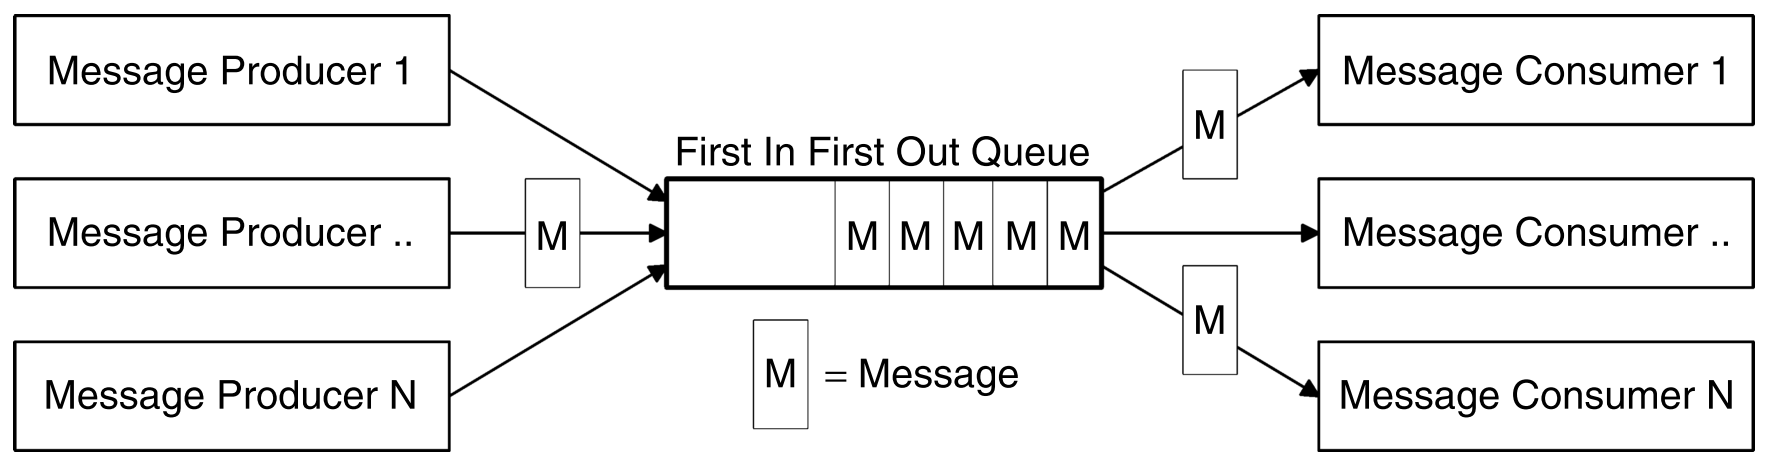
\includegraphics[width=.8\textwidth]{images/middleware_queue.png}
%     \caption{A Scenario where Queue is used as Message-Oriented Middleware}
%     \label{fig:diagram}
% \end{figure}

The abstract syntax tree of \emph{system}s is as follows:
\begin{bnf}
    \ntsym{system} ::= & \tsym{system} \ntsym{template}^?\ntsym{identifier} \tsym{(} \ntsym{port}^* \tsym{)} \tsym{\{}\\
    & (\tsym{internals} \ntsym{identifier}^+)^? \\
    & (\tsym{components} \tsym{\{} \ntsym{componentDecl}^* \tsym{\}})^? \\
    & \tsym{connections} \tsym{\{} \ntsym{connectionDecl}^* \tsym{\}} \tsym{\}}\\
    \ntsym{componentDecl} ::= & \ntsym{identifier}^+ \tsym{:} \ntsym{systemType} \\
    \ntsym{connectionDecl} ::= & \ntsym{systemType} \ntsym{params} \tsym{(} \ntsym{portName}^+ \tsym{)}
\end{bnf}

% The \emph{type} of a system (i.e. its template, name, and ports) shares exactly the same form and meaning with \emph{type} of an automaton. This also suggests that system is NOT a special semantics unit, but simply an compositional approach to pile up automata.
% We declare a system with its template, name and type, then it is implemented by an optional set of \emph{internal node}s, an optional set of \emph{component}s and a set of \emph{connection}s.

\smalltitle{Template} In templates of systems, all the parameter types being supported include: \emph{a)} parameters of abstract type \texttt{type}, \emph{b)} parameters of primitive types and composite types, and \emph{c)} interfaces and functions.

\smalltitle{Name and Type} Exactly the same as \emph{name} and \emph{type} of an automaton.

\smalltitle{Components} In \texttt{components} segments, we can declare any entity of an \emph{interface type} as components, e.g. an automaton, a system, or a parameter of interface type. 
Ports of a component can be referenced by \texttt{identifier.portName} once declared.

\smalltitle{Connections} Connections, e.g. the queue in Fig. \ref{fig:diagram}, are used to connect \emph{a) the ports of the system itself, b) the ports of its components, and c) the internal nodes}. We declare the connections in \texttt{connections} segments.
Both components and connections are supposed to run as automata in parallel.

\smalltitle{Internals} \liyi{Sometimes we need to combine multiple connections to perform more complex coordination behavior. Internal nodes, declared in \texttt{internals} segments, are untyped identifiers which are capable to weld two ports with consistent data-flow direction. For example, in Fig.~\ref{fig:diagram} the two internal nodes (denoted by $\bullet$) are used to combine a \emph{replicator}, a queue and a \emph{merger} together to work as a multi-in-multi-out queue.}


% Essentially, data flow in an internal node should always follow the same direction, i.e. an internal node doesn't collect or generate any data, it only receives from one end and forward it simultaneously. The direction, together with the type of an internal node, should be determined when being compiled.

A system is denoted by a 4-tuple
$S=\langle Ports, Entities, Internals, Links\rangle$ where $Ports$ is a set of ports, $Entities$ is a set of automata or systems (including both components and connections), $Internals$ is a set of internal nodes and $Links$ is a set of pairs, where each element of such a pair is either a port or an internal node. A link $\langle p_1,p_2\rangle$ suggests that $p_1$ and $p_2$ are linked together. A well-defined system satisfies the following assumptions:

% TODO:
\begin{enumerate}
    \item $\forall \langle p_1,p_2\rangle \in Links$, data transfer from $p_1$ to $p_2$. For example, if $p_1\in Ports$ is an input port, $p_2$ could be
    \begin{itemize}
        \item an output port of the system ($p_2\in Ports$), 
        \item an input port of some automaton $A_i\in Automata$ ($p_2\in A_i.Ports$), or
        \item an internal node ($p_2\in Internals$).
    \end{itemize}
    \item $\forall n\in Internals,\exists!p_1,p_2$, s.t. $\langle p_1,n\rangle ,\langle n,p_2\rangle\in Links$ and $p_1,p_2$ have the same data type.
\end{enumerate}

\begin{example}[\lang{} Model of the System in Fig. \ref{fig:diagram}] In Fig. \ref{fig:diagram}, a simple scenario is presented where a queue is used as a message-oriented middleware. To model this scenario, we need two automata \emph{Producer} and \emph{Consumer} (details are omitted due to space limit, and can be found at \cite{medmodels}) that produce or consume messages of type \emph{T}.
\begin{lstlisting}
automaton <T:type> Producer (OUT: out T) { ... }
automaton <T:type> Consumer (IN: in T) { ... }

system <T:type> middleware_in_use () {
    components {
        producer_1, producer_2, producer_3 : Producer<T>;
        consumer_1, consumer_2, consumer_3 : Consumer<T>;
    }
    internals  M1, M2 ;
    connections {
        Merger<T>(producer_1.OUT, producer_2.OUT, producer_3.OUT, M1);
        Queue<T>(M1, M2);
        Replicator<T>(M2, consumer_1.IN, consumer_2.IN, consumer_3.IN);
    }
}
\end{lstlisting}
\label{exp:middleware_system}
\end{example}
\section{Semantics}
\label{sec:semantics}

\subsection{Configurations of Automata}
\label{subsec:config}
% TODO: formalization of adjoint variables
Configurations are used to represent the state of an automaton. Since we don't have locations here, it only depends on the values of its locally accessible variables, which includes both \emph{adjoint variables} and \emph{local variables}.

\begin{definition}[Valuation]
An evaluation of a set of variables $Vars$ is defined as a function $v$ that satisfies $\forall x\in Vars,v(x)\in Dom(type(x))$. We denote all the possible evaluations of a variable set $Vars$ as $Val(Vars)$.
% TODO: how to say `without confusion`
\end{definition}

\begin{definition}[Configuration] A configuration of an automaton $A=\langle Ports,$ $Vars,Trans_G\rangle$ is defined as a tuple $(v_{loc},v_{adj})$ where $v_{loc}\in Val(Vars)$ is a valuation on local variables, and $v_{adj}\in Val(Adj(P))$ is a valuation on adjoint variables. 
\end{definition}

\subsection{Canonical Form of Transitions}
\label{subsec:canonical}

% TODO: what features?
% As mentioned before, transitions in an automaton have fantastic features to write simple but powerful models, including \emph{a) Priority}. In this subsection we introduce how these features work, and how to convert the rich-featured models to traditional ones.
\begin{definition}[Canonical Transitions]
A transition $t=g\rightarrow\{s_1,\cdots,s_n\}$ is canonical iff. its statements $\{s_i\}$ is an interleaving sequence of assignments and performs which start from an assignment, e.g. \texttt{a:= exp$_1$; perform A; b:= exp$_2$; $\cdots$}.
\end{definition}
We only need to simple steps to canonicalize a transition, they are:
\begin{enumerate}
    \item Merging the contiguous assignments. As mentioned before, an assignment statement is represented as a function $f:EV\rightarrow EV$. Thus a list of multiple assignments $f_1,\cdots, f_n$ can be simplified by $f=f_1\circ\cdots \circ f_n$.
    \item Any two adjacent performs should be separated by a identical assignment $id_{EV}$. 
\end{enumerate}

\smalltitle{Observable} A transition is always \emph{observable}, i.e. it will makes some difference to the context. For example, without this assumption, a transition \texttt{true -> x := x} will block the whole model by endless meaningless executions.

\begin{definition}[Canonical Transition Groups]
    A transition group is canonical iff. it only contains one canonical transition.
\end{definition}

\smalltitle{Priority} Given a set of ordered transitions.
\[
    \{g_1\rightarrow S_1,g_2\rightarrow S_2,\cdots,g_n\rightarrow S_n\}
\]
As required by the \emph{priority} assumption, a transition can be fired only if all the previous ones are not enabled (i.e. their guards are not satisfied) yet. In \lang{}, this feature is resolved simply by adding $\lnot g_i$ to all $g_j(j>i)$. E.g.
\[
    \{g_1\rightarrow S_1, g_2\land(\lnot g_1)\rightarrow S_2,\cdots,g_n\land(\lnot g_1\land \lnot g_2\land\cdots\land \lnot g_{n-1})\rightarrow S_n\}
\]
Now let's consider a set of ordered groups $t_{G_i}$, where $t_{G_i}$ contains $l_i$ transitions,
\begin{small}
\[
    T_G=\{t_{G_1}=\{g_{11}\rightarrow S_{11},\cdots, g_{1l_1}\rightarrow S_{1l_1}\},\cdots,t_{G_n}=\{g_{n1}\rightarrow S_{n1},\cdots,g_{nl_n}\rightarrow S_{nl_n}\}\}
\]
\end{small}
Informally speaking, once a transition in $t_{G_1}$ is enabled, all the other transitions in $t{G_i}(i>1)$ should be strictly prohibited from being fired. We use $enab(t_G)$ to denote the condition where at least one transition in $t_G$ is enabled, formalized as
\[
    enab(t_G=\{g_1\rightarrow S_1,\cdots, g_n\rightarrow S_n\}) = g_1\lor\cdots\lor g_n
\]
Then we can generate the new set of transitions with no dependency on priority:
\begin{eqnarray*}
    g_{11}\rightarrow S_{11},&\cdots&,g_{1l_1}\rightarrow S_{1l_1}, \\
    g_{21}\land \lnot enab(t_{G_1})\rightarrow S_{21}, &\cdots&, g_{2l_2} \land \lnot enab(t_{G_1})\rightarrow S_{2l_2}, \cdots \\
    g_{n1}\land \lnot enab(t_{G_1},\cdots,t_{G_{n-1}})\rightarrow S_{n1}, &\cdots&, g_{nl_n} \land \lnot enab(t_{G_1},\cdots,t_{G_{n-1}})\rightarrow S_{nl_n} \\
\end{eqnarray*}
where $enab(t_{G_1},\cdots,t_{G_{n-1}})$ is an abbreviation of $enab(t_{G_1})\lor\cdots\lor enab(t_{G_{n-1}})$. It indicates that at least one group in $t_{G_i}$ is enabled.
\subsection{From System to Automaton}
\label{subsec:composition}

Systems, as shown previously, are simply introduced to construct automata in a more natural way. Now we show how such a system can be flatten as a standard automaton.

% TODO: canonical form of a transition mus requires a interleaving form, may be filled
% with non-sense assignments
% TODO: topological sorting
\begin{algorithm}[H]
    \caption{Scheduling in a Synchronous Set of External Transitions}
    \label{alg:synchronize}
    \begin{algorithmic}[1]
        \REQUIRE $t_1,t_2,\cdots,t_n$ are transitions (canonical form)
        \ENSURE $t=\mbox{\texttt{Schedule}}(t_1,\cdots,t_n)$
        \IF{$\{t_i\}$ don't belong to different automata or $\exists t_i$ is internal}
            \STATE $t\leftarrow null$
            \RETURN
        \ENDIF
        \STATE \emph{t.g, t.S} $\leftarrow \bigwedge_i t_i.g,\:\{\}$
        \FOR{$i\leftarrow 1,\cdots,n$}
            \IF {$t_i.s_1$ is an \emph{assignment}}
            \STATE add $t_i.s_1$ to the head of $t.S$
            \ENDIF
            \STATE $p$ $\leftarrow$ the first \emph{perform} statement
            \WHILE {$p$ $\neq$ \emph{null}}
                \STATE $a\leftarrow$ the \emph{assignment} statement after $p$
                \STATE $p'\leftarrow$ the next \emph{perform} statement after $p$
                \IF {$p\in t.S$}
                    \STATE insert $a$ to $t.S$ exactly after $p$
                    \STATE remove $p$ from $t.S$
                \ENDIF
            \ENDWHILE
        \ENDFOR
        \STATE $t\leftarrow$ \texttt{Canonicalize($t$)}
    \end{algorithmic}
\end{algorithm}

\begin{algorithm}[H]
    \caption{Compose Several Automatons}
    \label{alg:compose}
    \begin{algorithmic}[1]
        \REQUIRE $A_1,A_2,\cdots,A_n$ are automata
        \ENSURE $A=\mbox{\texttt{Compose}}(A_1,\cdots,A_n)$
        \STATE rename local variables in $A_1,\cdots,A_n$ to avoid duplicated names
        \STATE $A \leftarrow $ empty automaton
        \STATE $ext\_trans\leftarrow \{\}$
        \FOR{$i\leftarrow 1,2,\cdots,n$}
            \STATE add all local variables of $A_i$ to $A$
            \STATE add all internal transitions of $A_i$ to $A$
            \STATE add all external transitions of $A_i$ to $ext\_trans$
        \ENDFOR
        \FOR{$set\_trans\leftarrow$ subset of $ext\_trans$}
            \STATE $newedge\leftarrow \mbox{\texttt{Schedule}}(set\_trans)$ 
            \IF{\emph{newedge $\neq$ null}}
                \STATE add \emph{newedge} to $A$
            \ENDIF
        \ENDFOR
    \end{algorithmic}
\end{algorithm}

\subsection{Automaton as Labelled Transition System}

\begin{definition}[Transition System, TS]
    A transition system is a tuple $(S,\rightarrow)$ where $S$ is a set of states and $\rightarrow\subseteq S\times\Sigma\times S$ is a set of transitions. For simplicity reason, we use $s\rightarrow s'$ to denote $(s,s')$ in $\rightarrow$.
\end{definition}

Suppose $A=\langle Ports, Vars, Trans_G\rangle$ is an automaton, its semantics can be captured by a labelled transition system $\langle S_A, \rightarrow_A\rangle$ where
\begin{itemize}
    \item $S_A$ is the set of all configurations of $A$.
    \item $\rightarrow_A\subseteq S_A\times \Sigma_A\times S_A$ is a set of transitions constructed by the following rules.
\end{itemize}

\begin{mathpar}
    \inferrule* [right=R-InputStatus] {p\in P_{in}}{(v_{loc}, v_{adj})\xrightarrow{}_A(v_{loc},v_{adj}[p.reqWrite\mapsto \lnot p.reqWrite])} \\
    \inferrule* [right=R-InputValue] {p\in P_{in}, val\in type(p.value)}{(v_{loc}, v_{adj})\xrightarrow{}_A(v_{loc},v_{adj}[p.value\mapsto val])} \\
    \inferrule* [right=R-OutputStatus] {p\in P_{out}}{(v_{loc}, v_{adj})\xrightarrow{}_A(v_{loc},v_{adj}[p.reqRead\mapsto \lnot p.reqRead])} \\
    \inferrule* [right=R-Internal] {\{g\rightarrow \{s\}\}\in Trans_G\mbox{ is internal}}{(v_{loc}, v_{adj})\xrightarrow{}_A s(v_{loc},v_{adj})} \\
    \inferrule* [right=R-External] {\{g\rightarrow S\}\in Trans_G\mbox{ is external, } \{s_1,\cdots,s_n\}\mbox{ are the assignments in $S$}}{(v_{loc}, v_{adj})\xrightarrow{}_A s_n\circ\cdots\circ s_1(v_{loc},v_{adj})} \\
\end{mathpar}

The first three rules describe the potential change of context, i.e. the adjoint variables. R-InputStatus and R-OutputStatus shows that the reading status of an output port and status of an input port may changed randomly. And R-InputValue shows that the value of an input port may be updated by the context.

The rule R-Internal models the internal transitions in $Trans_G$. As illustrated previously, an internal transition doesn't contains any perform statement. So its canonical form comprises only one assignment $s$. Firing such a transition will simply apply $s$ to the current configuration.

Meanwhile, R-External models the external transitions, where the automaton need to interact with its context. Fortunately, since all the context change are captured by the first three rules, we can simply regard the context as a set of local variables. Consequently, the only difference between an internal transition and an external transitions is that the later may contains multiple assignments.

%TODO: take queue as an example
\section{Case Study}
\label{sec:casestudy}

In modern distributed computing frameworks (e.g. MPI\cite{mpibook} and ZooKeeper\cite{JunqueiraZab2011}), \emph{leader election} plays an important role to organize multiple servers efficiently and consistently. This section shows how a classical leader election algorithm is modeled and reused to coordinate other components in \lang{}.

\cite{HagitDistributed2004} proposed a classical algorithm for a typical leader election scenario, as shown in Fig. \ref{fig:leaderelection}. Distributed processes are organized as an \emph{asynchronous unidirectional} ring where communication takes place only between adjacent processes and following certain direction (indicated by the arrows on edges in Fig. \ref{fig:leaderelection} (a)).

\begin{figure}
	\centering
	\resizebox{.8\textwidth}{!}{
        \tikzstyle{node}=[
    circle,
    draw
]

\begin{tikzpicture}[remember picture]
    \def \n {5}
    \def \radius {2cm}
    \def \margin {11} % margin in angles, depends on the radius

    \foreach \s in {1,...,\n}
    {
    \node[draw, circle] at ({360/\n * (\s - 1)}:\radius) {$P_\s$};
    \draw[<-, >=latex] ({360/\n * (\s - 1)+\margin}:\radius) 
        arc ({360/\n * (\s - 1)+\margin}:{360/\n * (\s)-\margin}:\radius);
    }

    \node[draw, rectangle, minimum width=4cm] at (6,0) {
        \begin{tabular}{c}
            \\
            Process ($P_i$) \\
             \\
            \begin{tikzpicture}[remember picture]
                \node [draw, rectangle, minimum width=3cm, minimum height=1cm] (connector) at (0,0) {\texttt{election\_module}};
            \end{tikzpicture} \\
            \\
            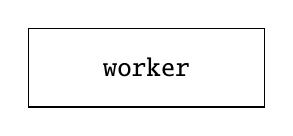
\begin{tikzpicture}[remember picture]
                \node [draw, rectangle, minimum width=3cm, minimum height=1cm] (component) at (0,0) {\texttt{worker}};
            \end{tikzpicture}
            \vspace{0.5em}
        \end{tabular}
        };
    
    \draw[->, >=latex] (3,0.3) -- (connector) node[midway, above, xshift=-0.35cm] {\texttt{left}} ;
    \draw[->, >=latex] (connector) -- (9,0.3) node[midway, above, xshift=0.3cm] {\texttt{right}};
    \draw[<->, >=latex] (component) -- (connector) ;

    \node[] at (0,-2.8) {(a)};
    \node[] at (6,-2.8) {(b)};
\end{tikzpicture}
    }
	\caption{(a) Topology of an Asynchronous Ring and (b) Structure of a Process}
	\label{fig:leaderelection}
\end{figure}

The algorithm has the following steps:
\begin{enumerate}
	\item Each process sends a voting message including its own \emph{id} to its successor.
	\item A process, when receives a voting message, will
	\begin{itemize}
		\item forward the message to its successor if it contains a larger \emph{id} than itself,
		\item ignore the message if it contains a smaller \emph{id} than itself, and
		\item take itself as a leader if it contains the same \emph{id} with itself, and send an acknowledgement message to this successor, which will be spread over around the ring.
	\end{itemize} 
\end{enumerate}

Here we formalize this algorithm through a more general approach. Leader election is encapsulated as the \texttt{election\_module}. A computing module \texttt{worker},  attached to the \texttt{election\_module}, is an implementation of the working process. 

Two types of messages, \texttt{msgVote} and \texttt{msgLocal}, are supported when formalizing this architecture. Voting messages \texttt{msgVote} are transferred between the processes. A voting message carries two fields, \emph{vtype} that declares the stage of leader election (either it is still voting or some process has already been acknowledged) and \emph{id} is an identifier of the current leader (if it exists). On the other hand, \texttt{msgLocal} is used when a process communicates with its corresponding worker.
\begin{example}[The Election Module] The following automaton shows how the election algorithm is implemented in \lang{}. Due to the space limit, we omit some transitions here. A full version can be found at \cite{medmodels}.
\begin{lstlisting}[basicstyle=\scriptsize\ttfamily]
automaton <id:int> election_module ( left : in msgVote, right : out msgVote,
	query : out msgLocal
) {
	variables {
		leaderStatus : enum { pending, acknowledged } init pending;
		buffer : (voteMsg | NULL) init {vtype: vote, id:id};
		leaderId : (int | NULL) init null;
	}
	transitions {
		(buffer != null)&&(buffer.vtype == vote)&&(buffer.id < id) -> {buffer := null;}
		(buffer != null)&&(buffer.vtype == vote)&&(buffer.id == id) -> {buffer.vtype := ack;}
		(buffer != null)&&(buffer.vtype == ack)&&(buffer.id < id) -> {
			// restart voting if the acknowledged leader has a smaller id
			buffer := { vtype: vote, id: id };
		}
		(buffer != null)&&(buffer.vtype == ack)&&(buffer.id >= id) -> {
			leaderStatus := acknowledged;
			leaderId := buffer.id;
			buffer := buffer.id == id ? null : buffer;
		}
	}
}
\end{lstlisting}
\end{example}


The following code fragment encodes a parallel program containing 3 \emph{worker}s and 3 \emph{election\_module}s to organize the \emph{worker}s. It is a simplified version of the one in Fig. \ref{fig:leaderelection}. In this example, we do not focus on the implementation details on \emph{worker}s. Instead, we hope that any component with a proper interface could be embedded into this system. Consequently \emph{worker} is taken as a parameter of interface type.

\begin{lstlisting}[basicstyle=\scriptsize\ttfamily]
system <worker: interface (query:in msgLocal)> parallel_instance() {
	components {
		E1 : election_module<1>;
		E2 : election_module<2>;
		E3 : election_module<3>;
		C1, C2, C2 : worker;
	}	
	connections {
		Sync<msgVote>(E1.left, E2.right);
		Sync<msgVote>(E2.right, E3.left);
		Sync<msgVote>(E3.right,	E1.left);
		
		Sync<msgLocal>(C1,query,  E1.query);
		Sync<msgLocal>(C2,query,  E2.query);
		Sync<msgLocal>(C3,query,  E3.query);
	}
}
\end{lstlisting}

As we are modeling the leader election algorithm on a synchronous ring, only synchronous communication channels \emph{Sync}s are involved in this example. The implementation details of \texttt{Sync} can be found in  \cite{medmodels}.

\section{Conclusion and Future Work}
\label{sec:conclusion}

A new modeling language \lang{} is proposed in this paper to help with component-based software engineering through a formal way. With the basic behavior unit \emph{automata} that captures the formal nature of components and connections, and \emph{systems} for hierarchical composition, the language is easy-to-use for both formal method researchers and system designers.

This paper is a preface of a set of under-development tools. We plan to build a model checker for \lang{}, and extend it through symbolic approach. An automatic code-generator is also being built to generate platform-specific codes like \emph{Arduino}\cite{margolis2011arduino}.

\section*{Acknowledgements}

The work was partially supported by the National Natural Science Foundation of China under grant no. 61532019, 61202069 and 61272160.

\bibliographystyle{splncs03}
\bibliography{fm,local}

\newpage
\section*{Appendix}

\setcounter{theorem}{0}
\begin{theorem}[Equivalence between Schedules] If two set of assignment statements $S_1, S_2$ are generated from the same set of external transitions, they have exactly the same behavior (i.e. execution of $S_1$ and $S_2$ under the same configuration will lead to the same result.
\end{theorem}
\begin{proof}
    Apparently, when executing statements, all the changes on configurations come from \emph{assignments}. Once we successfully prove that for each assignment, its pre-configuration and post-configuration in $S_1$ and $S_2$ are exactly the same, we are able to finish this proof.
    
    In the following proof, we denote $S_1$ and $S_2$ by $S_1=\{s_1,\cdots,s_n\},S_2=\{s'_1,\cdots,s'_n\}$, and the automaton that a transition belongs to by $Automaton(s)$.
    \begin{enumerate}
        \item Let's come to the \emph{FIRST} assignment state $s$ in $S_1$ where shared variables is assigned. We assume that its corresponding statement in $S_2$ is $s'$. Comparing $s$ and $s'$, we have:
        \begin{enumerate}
            \item $s'$ is also the first assignment in $S_2$ which modifies \emph{this set} of variables.
            \emph{(A shared variable can be assigned in one of its owner, thus all assignments that modifies this variable belong to the same transition, and their order is strictly maintained.)}
            \item $s$ and $s'$ include no reference to other shared variables. \emph{(A shared variable can be dereferenced only when it has been assigned before, however $s$ is the first assignment which modifies a shared variable.)}
            \item In the pre-configuration of $s$ and $s'$, all the local variables of $Automaton(s)$ have the same evaluation. \emph{(Derived from the same reason in (a))}.
        \end{enumerate}
        Consequently, in the post-configuration of $s$ and $s'$, all the shared variables have the \emph{SAME} evaluation.

        \item Assume that all assignments (to shared variables) in $s_1,\cdots,s_i$ have been proved that satisfy the proposition, now we are going to prove that $s$, the first transition where shared variables are dereferenced in $s_{i+1},\cdots,s_n$ and its corresponding $s'$ also satisfy it.
    \end{enumerate}
\end{proof}

\end{document}